\section{Evaluation}
\subsection{Energyspectrum}

\begin{figure}[htpb]
    \centering
    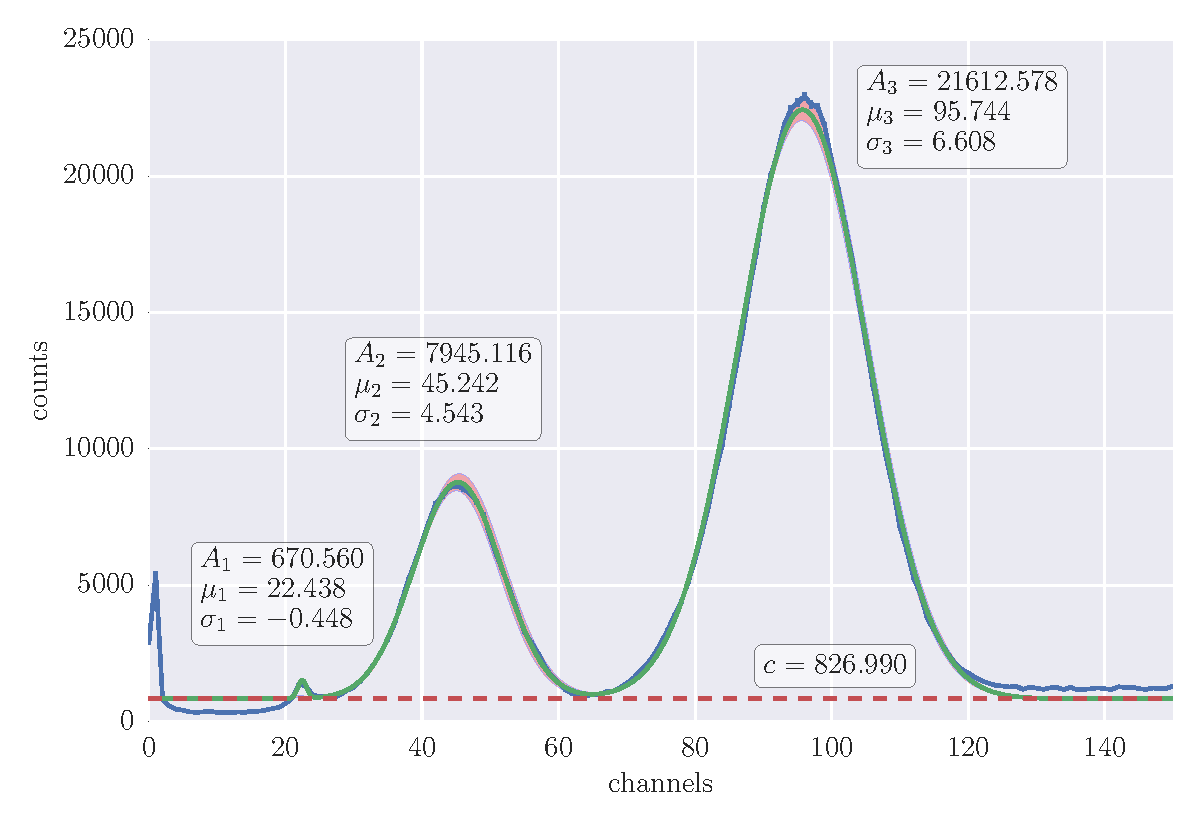
\includegraphics[width=1.1\linewidth]{analysis/figures/plot6_3_reg}
    \caption{These are the fitting curves of the ameritium spectrum with respect to gaussian distributions:
        $A_1\exp{\left[\frac{(x-\mu_1)^2}{2 \sigma_1^2} \right]}+
         A_2\exp{\left[\frac{(x-\mu_2)^2}{2 \sigma_2^2} \right]}+
         A_3\exp{\left[\frac{(x-\mu_3)^2}{2 \sigma_3^2} \right]}+ c$}
         \label{fig:name}
\end{figure}

\begin{figure}[htpb]
    \centering
    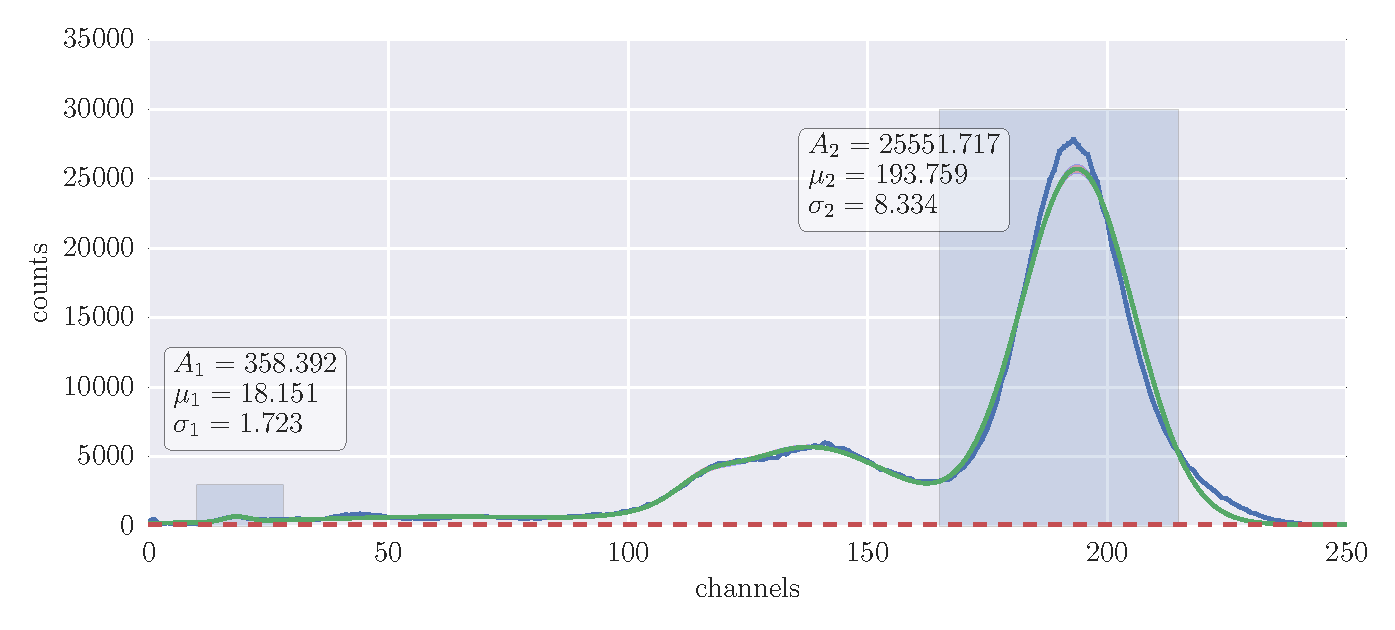
\includegraphics[width=1.1\linewidth]{analysis/figures/plot2_1a_reg}
    \caption{These are the fitting curves of the ameritium spectrum with respect to gaussian distributions:
        $A_1\exp{\left[\frac{(x-\mu_1)^2}{2 \sigma_1^2} \right]}+
         A_2\exp{\left[\frac{(x-\mu_2)^2}{2 \sigma_2^2} \right]}+
         A_3\exp{\left[\frac{(x-\mu_3)^2}{2 \sigma_3^2} \right]}+ 
         A_4\exp{\left[\frac{(x-\mu_4)^2}{2 \sigma_4^2} \right]}+ c$
         The exponents of $A_3$ and $A_4$ will not be given, since we do not use them.}
         \label{fig:name}
\end{figure}



\begin{figure}[htpb]
    \centering
    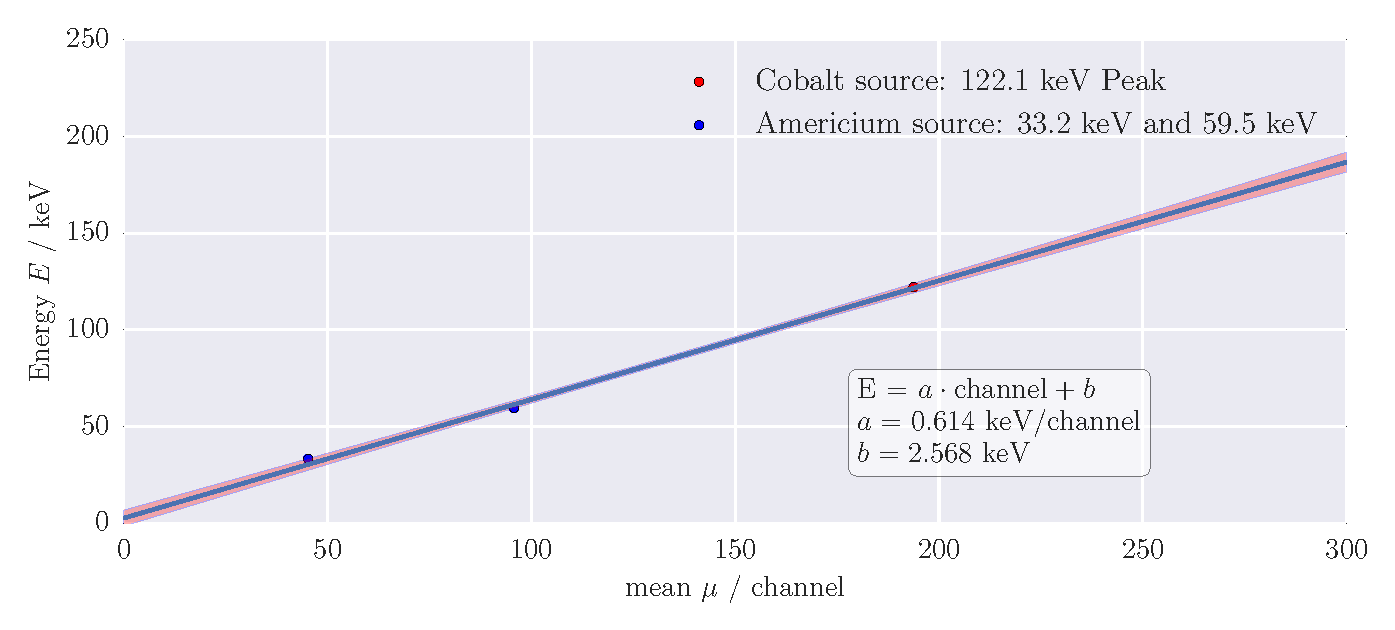
\includegraphics[width=1.0\linewidth]{analysis/figures/plot_E}
    \caption{Name}
    \label{fig:name}
\end{figure}
\subsubsection{Calibration of TAC-MCA Signal}
\label{subs:calib_TAC}
In order to relate the channels to the delay, we used the following
measurement for calibration. We used a least square fit for the parameters
of the linear relation:
\begin{align}
    \label{eq:coeff}
    y &= ax + b \\
    a &= \left[ 1.315 \pm 0.005 \right] \mathrm{ns} / \mathrm{Channel}\\
    b &= \left[ -22.6 \pm 0.5 \right]\mathrm{ns} 
\end{align}
where the $x$-values are given by the number of the corresponding channel. 
The resulting covariance matrix of the fit is the following:
\begin{align}
    \label{eq:cov}
    \mathrm{cov}(a, b) &=& 
    \begin{pmatrix}
        2.318 \cdot 10^{-5}\mathrm{ns}^2 &-2.089\cdot 10^{-3}\mathrm{ns}^2\\
        -2.089\cdot 10^{-3}\mathrm{ns}^2&2.328\cdot 10^{-1}\mathrm{ns}^2\\
    \end{pmatrix}
\end{align}
where the units correspond to those of $a$ and $b$ 
(e.~g. $\mathrm{cov}(a,a) = 2.318\mathrm{e}-05 \mathrm{ns^2} / \mathrm{Channel}^2$).
The $\chi^2$-test results in:
\begin{align}
    \label{eq:}
   \chi^2 = 0.972
\end{align}

\label{sub:calibration_of_tac_mca_signal}
\begin{figure}[htpb]
    \centering
    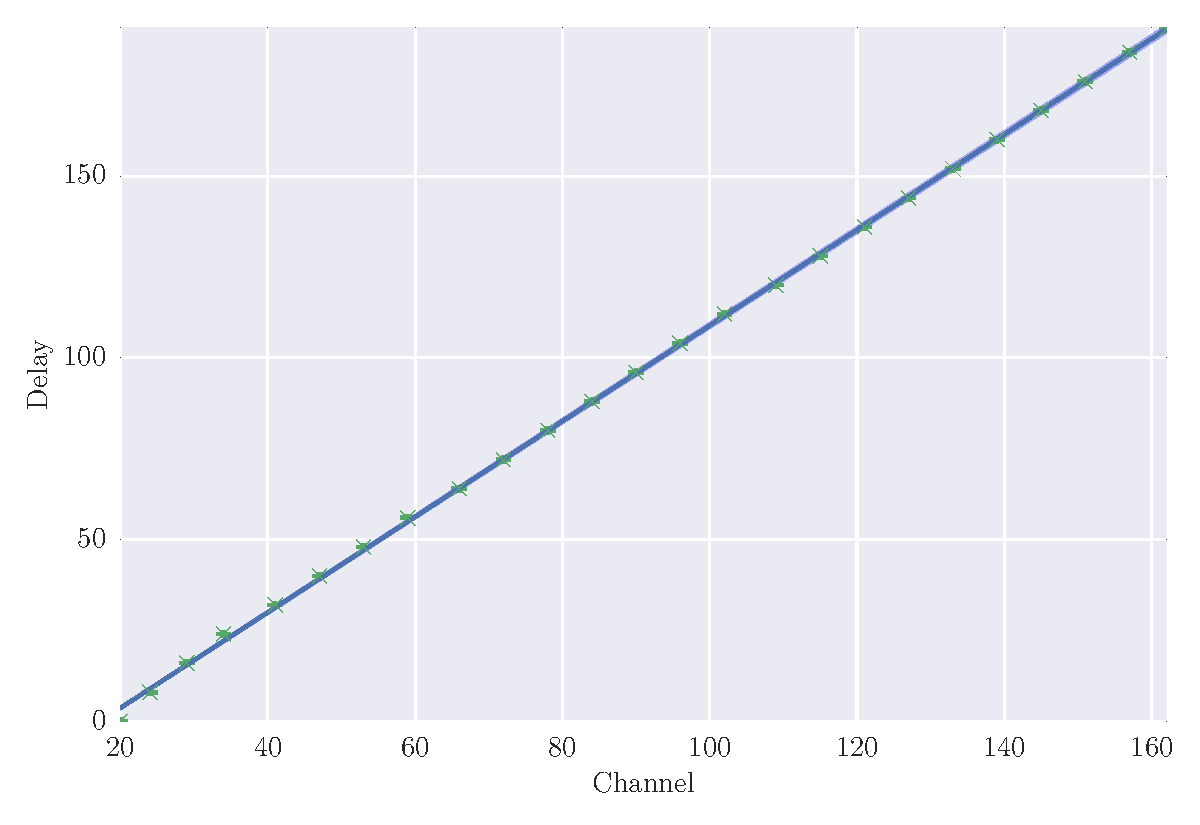
\includegraphics[width=1.0\linewidth]{analysis/figures/plot7}
    \caption{Calibration of the TAC-MCA Signal. The errorbars are too small
        to see clearly, since the $\chi^2$ test ist also nearly 1.}
    \label{fig:plot7}
\end{figure}



\subsection{Naive approach: Ad-hoc solution}
In this section we will make use of the previous sections: Forwarding the channel to the time regime and
reducing the background from our main figure in order to evaluate the half life period.\\\\
The measurement of randomized concidences lasted 4.1 lasted \textbf{6080 seconds} = 1 hour 41 minutes and 20 seconds, while
the measurement of delayed coincidences lasted \textbf{52658 seconds} =  14 hours, 37 minutes and 38 seconds. 
In order to compensate for this disparity, we need to extrapolate the background by the following
\begin{equation}
\mathrm{\textbf{total:} } \quad 79 \quad \mathrm{events} \quad \Rightarrow 5.177\cdot 10^{-5}\quad \mathrm{events/ (channel \cdot second)}
\end{equation}
If we extrapolate this for the delayed coincidences, we arrive at
\begin{align}
\begin{split}
\mathrm{\textbf{background estimate:} } \quad  5.177\cdot 10^{-5} \cdot 52658 \quad \mathrm{events / channel} \\
= 2.726\quad \mathrm{events/ channel}
\end{split}
\end{align}
Now we 

\begin{figure}[htpb]
    \centering
    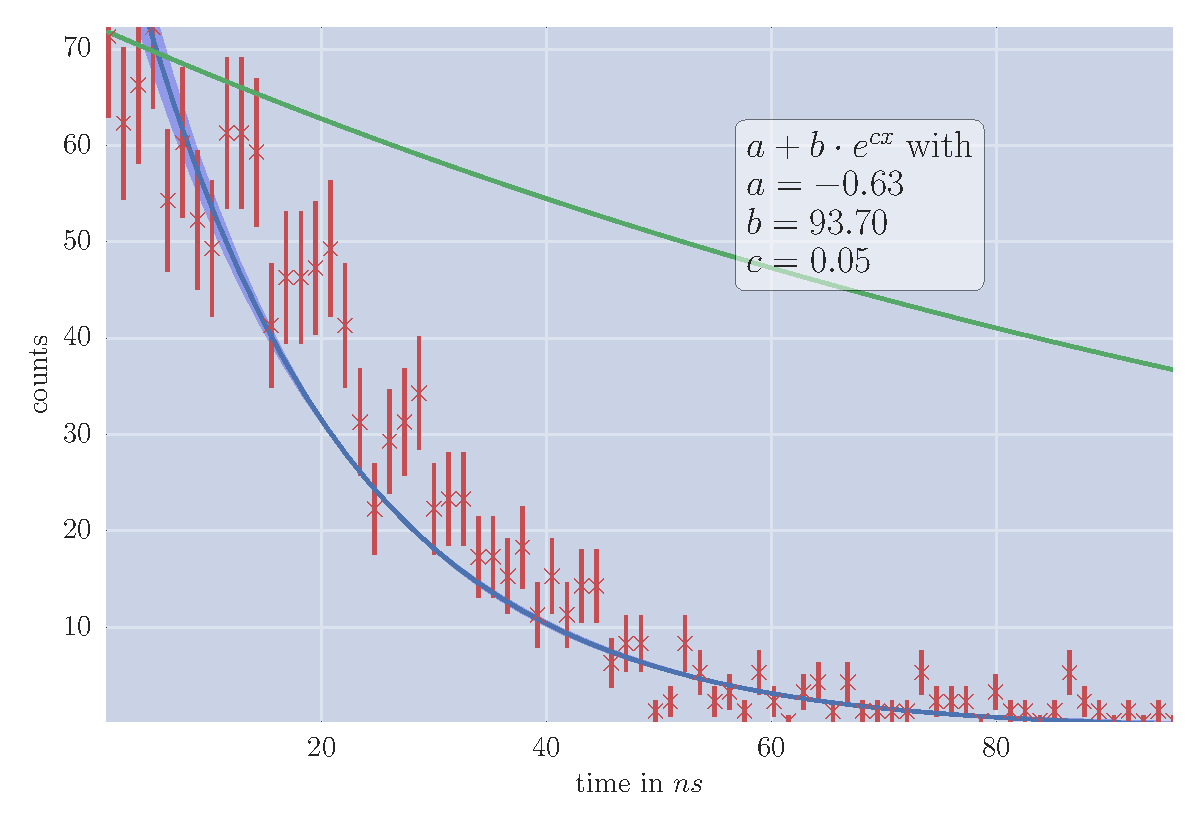
\includegraphics[width=0.8\linewidth]{analysis/figures/plot4_1_reg}
    \caption{Name}
    \label{fig:name}
\end{figure}




